\documentclass[a4paper]{article}
\usepackage[utf8]{inputenc}
\usepackage{graphicx}
\usepackage{amsmath}
\usepackage{listings}
\usepackage{color}
\usepackage{breqn}
\usepackage{geometry}
 \geometry{
 a4paper,
 total={150mm,257mm},
 left=30mm,
 top=20mm,
 }

\title{Akima sub-spline interpolation}
\author{René Munk Thalund}
\date{June 2022}

\begin{document}
\maketitle

\section{Introduction}

We seek to implement the Akima sub-spline interpolations method in \texttt{C\#}. The Akima sub-spline are cubic sub-splines, that seeks to alleviate some of the shortcomings of regular cubic splines while sacrificing continuity of the second derivative of the interpolation function. Furthermore since the polynomial coefficients for each segment are calculated using only a few input points locally around the segment, the Akima sub splines can be constructed without the large equation set, Gauss elimination and back-substitution needed in for cubic splines. Array indexing corresponding to the source code used below.

\section{Basic construction}
The piece-wise polynomials used on a set of $n$ input points, $(x_i,y_i)$, with $n = 0,1, \ldots,n-1$ have the form:
\begin{equation}
    A_i(x) = a_i + b_i(x-x_i) + c_i(x-x_i)^2 + d_i(x-x_i)^3
\end{equation}
It's helpful to define the $x$-increments and slopes:
\begin{align}
    h_i &= x_{i+1} - x{i} \\
    p_i &= \frac{y_{i+1} - y{i}}{h_i}, \text{ both with } n = 0,1, \ldots,n-2
\end{align}
The first derivatives $A_i'(x) = b_i$, are found using a weighed average of slopes of neighbouring input points;

\begin{align}
    b_i &= \frac{w_{i}p_{i-1} + w_{i-2}p_{i}}{w_{i+1}+w_{i-1}}, \text{ if } w_{i}+w_{i-2} \neq 0  \nonumber \\
    b_i &= \frac{p_{i-1}+p_i}{2}, \text{ otherwise}
    \label{eq:b_formula}
\end{align}
The weights are given by $w_i = |p_{i+1}-p_i|$. The quadratic and cubic coiffecients are then calculated as:
\begin{equation}
    a_i = y_i,\,c_i = \frac{2p_i - 2b_i - b_{i+1}}{h_i} \text{  and  } d_i = \frac{b_i + b_{i+1}-2p_i}{h_i^2}
\end{equation}



\section{Slope at end-points}
The formula \ref{eq:b_formula} for $b_i$, the spline's tangent slope at $(x_i,y_i)$ relies two adjacent input points on either side and hence doesn't work for $b_0, b_1, b_{n-2}$ and $b_{n-1}$. My implimentation offers three different schemes for the four end-point slopes:

\subsection{Naive end-points}
As suggested in the course notes, and the Wiki page on Akima sub-splines, the four slopes can naively be chosen as:
\begin{equation}
    b_0 = p_0,\,b_1 = \frac{p_0 + p_1}{2},\,b_{n-2} = \frac{p_{n-3} + p_{n-2}}{2} \text{ and } b_{n-1} = p_{n-2}
\end{equation}

\subsection{Akima end points}
Akima suggested adding four supplementary slopes $p_{-2}, p_{-1}, p_{n-1}$ and $p_{n}$ to be constructed as:
\begin{equation}
    p_{-2} = 3p_0-2p_1,\, p_{-1} = 2p_0-p_1,\, p_{n-1} = 2p_{n-2} - p_{n-3} \text{ and } p_{n} = 3p{n-2} - 2p{n-3}
\end{equation}
Given those, the entire set of $\{b_i\}$ can be calculated using equation \ref{eq:b_formula}. Comparing my \texttt{C\#} results with Python results, I found that this end-point scheme is the one used for the latter, see figure \ref{fig:5}.

\subsection{Bica's end points}
In a 2014 paper (https://doi.org/10.1016/J.CAGD.2014.03.001), A.M Bica devised a method so to minimise \emph{partial quadratic oscillation in average} (PQOA) in the intervals on the end sub-intervals $[x_0,x_2]$ and $[x_{n-3},x_{n-1}]$. The quite involved definitions on the PQOA is out of the scope, but I found it worthwhile to implement an option to use the four Bica-slopes, given by:

\begin{align}
    b_0 &= \frac{1}{\delta} \cdot \left[ \frac{y_1 - y_0}{4h_0} +
    \frac{9h_1^3\cdot b_2}{16(h_0^3+h_1^3)} +
    \frac{3h_0^2\cdot(y_1-y_0)}{16(h_0^3+h_1^3)} +
    \frac{3h_1^2\cdot(y_2-y_1)}{16(h_0^3+h_1^3)} \right ] \\ 
    b_1 &= \frac{1}{\delta} \cdot \left[ \frac{3h_1^3\cdot b_2}{4(h_0^3+h_1^3)} +
    \frac{7h_0^2\cdot(y_1-y_0)}{16(h_0^3+h_1^3)} +
    \frac{h_1^2\cdot(y_2-y_1)}{4(h_0^3+h_1^3)} \right], \text{ where}\\
    \delta &= \frac{7h_0^3+16h_1^3}{16(h_0^3+h_1^3)} \\ 
    b_{n-1} &= \frac{1}{\delta '} \cdot \left[ \frac{y_{n-1} - y_{n-2}}{4h_{n-2}} +
    \frac{9h_{n-3}^3 \cdot b_{n-3}}{16(h_{n-3}^3+h_{n-2}^3)} + 
    \frac{3h_{h-2}^2 \cdot(y_{n-2}-y_{n-1})}{16(h_{n-3}^3+h_{n-2}^3)} +
    \frac{3h_{n-3}^2\cdot(y_{n-3}-y_{n-2})}{16(h_{n-3}^3+h_{n-2}^3)} \right ] \\ 
    b_{n-2} &= \frac{1}{\delta '} \cdot \left[ \frac{3 h_{n-3}^3\cdot b_{n-3}}{4(h_{n-3}^3+h_{n-2}^3)} +
    \frac{7h_{n-2}^2\cdot (y_{n-1}-y_{n-2})}{16(h_{n-3}^3+h_{n-2}^3)} +
    \frac{h_{n-3}^2 \cdot (y_{n-2}-y_{n-3})}{4(h_{n-3}^3+h_{n-2}^3)}  \right], \text{ where} \\ 
    \delta ' &= \frac{7h_{n-2}^3+16h_{n-3}^3}{16(h_{n-3}^3+h_{n-2}^3)}
\end{align}
When comparing to the Bica paper, note that it considers $n+1$ input points (where I use $n$), and Bica indexes $h_i$ from 1 (where I index from 0 in order to maintain consistensy with the code.)

\section{Optimization}
\begin{itemize}
    \item After reading in the input data, the program calculates an array of coarse accumulated integration areas at the input x values. This array is kept and makes subsequent integration to interpoint x values faster.
    
    \item The last found binary search interval is kept, and checked as first option when a new integration point is requested. If z values all over the place are needed this adds two comparisons extra per if the next point is not in the same interval. However, when a large range of monotonic increasing or desceasing z values is requested – like when writing n consequtive z-values to the output file – it saves greatly on the search.
\end{itemize}

\section{Results}
I tested my Akima sub-spline routine on three strategic datasets. One with values of $sin(x)$, one with values of a step function and one with more arbitrary values, to check the difference in the three end-point schemes. The results are seen in figures \ref{fig:1} through \ref{fig:5}.

\begin{figure}
    \centering
    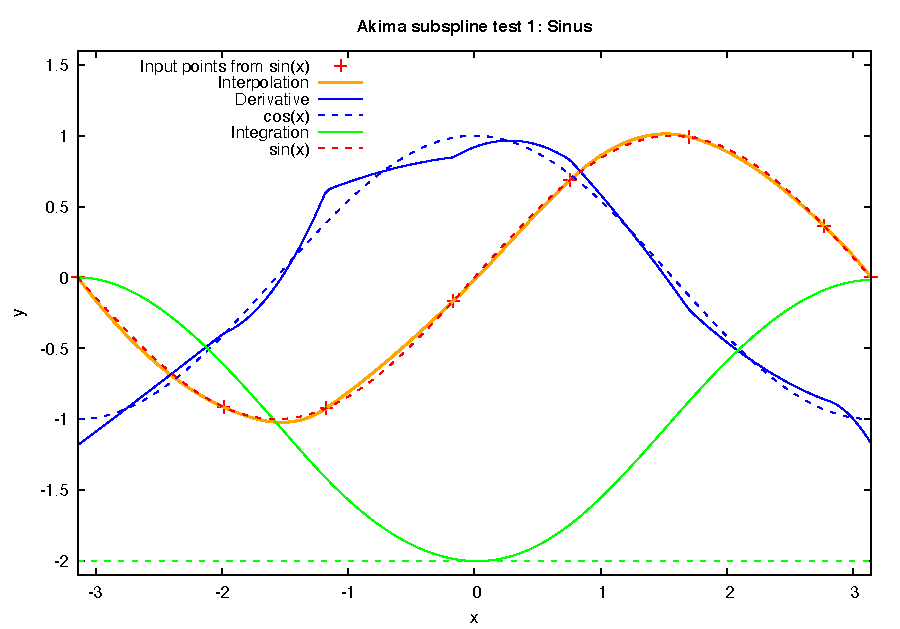
\includegraphics[width=0.9\textwidth]{fig/akima_spline_sin.pdf}
    \caption{Akima sub-splines on a dataset of $sin (x)$, with the $x$-values at irregular intervals. We notice that while the sub-spline (here using the Akima end point scheme) succeeds to connect the points smoothly, the resulting spline does not follow the mathematical sin(x) curve too well. The jagged line of the derivative (blue) is a tell-tell of the discontinuous second derivative – a trade-off to avoid the oscillating artefacts of cubic spline. The mathematical derivative $cos(x)$ plotted for reference. The integral (green) behaves more gently. Mathematically the anti-derivative of $sin(x)$ would reach -2 at $x=0$ and be back at $0$ at $x =\pi$ and this is replicated acceptably by the spline integration.}
    \label{fig:1}
\end{figure}

\begin{figure}
    \centering
    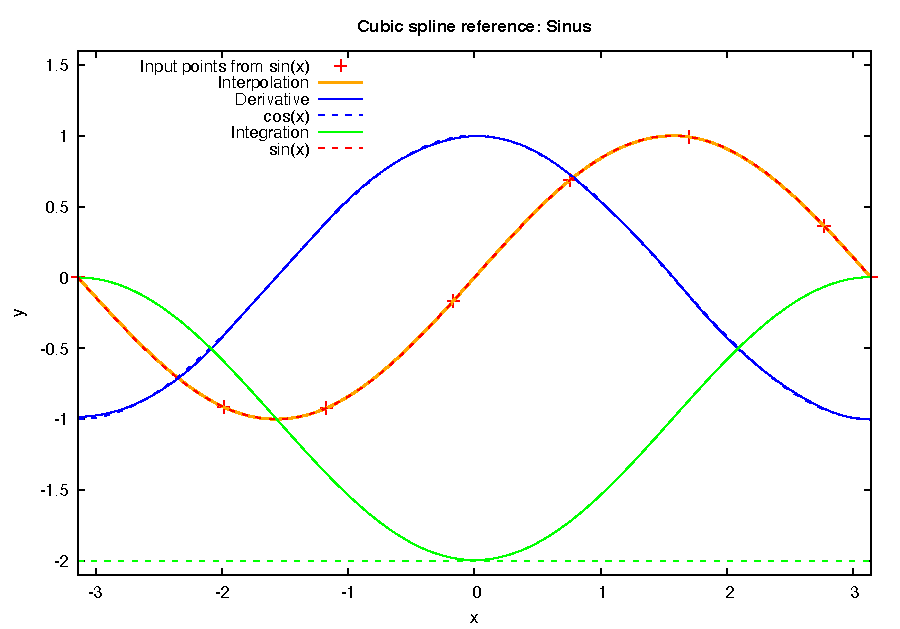
\includegraphics[width=0.9\textwidth]{fig/cubic_spline_sin.pdf}
    \caption{For reference my Cubic spline routine on the same dataset as in figure \ref{fig:1}. The cubic spline replicates $sin(x)$ and it's derivative excellently given just 8 input points over a full cycle.}
    \label{fig:2}
\end{figure}

\begin{figure}
    \centering
    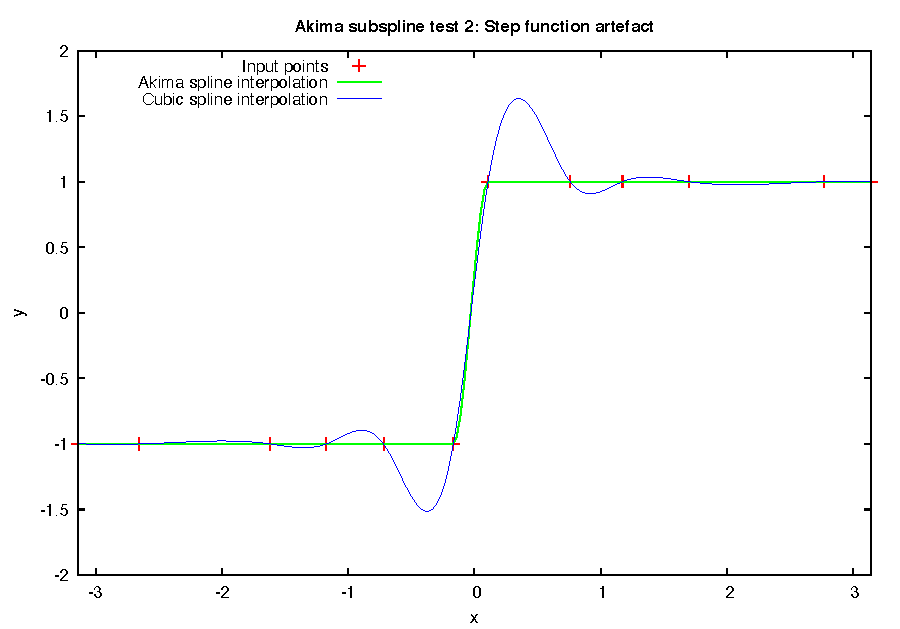
\includegraphics[width=0.9\textwidth]{fig/akima_spline_step.pdf}
    \caption{A data with a sudden step from -1 to 1 and otherwise constant values dementrates the advantage of Akima sub-splines. While the cubic spline interpolation (blue) has damped oscillations on either side of the jump, the akima sub-splines (green) stays constant besides on the interval with the actual step.}
    \label{fig:3}
 \end{figure}

\begin{figure}
    \centering
    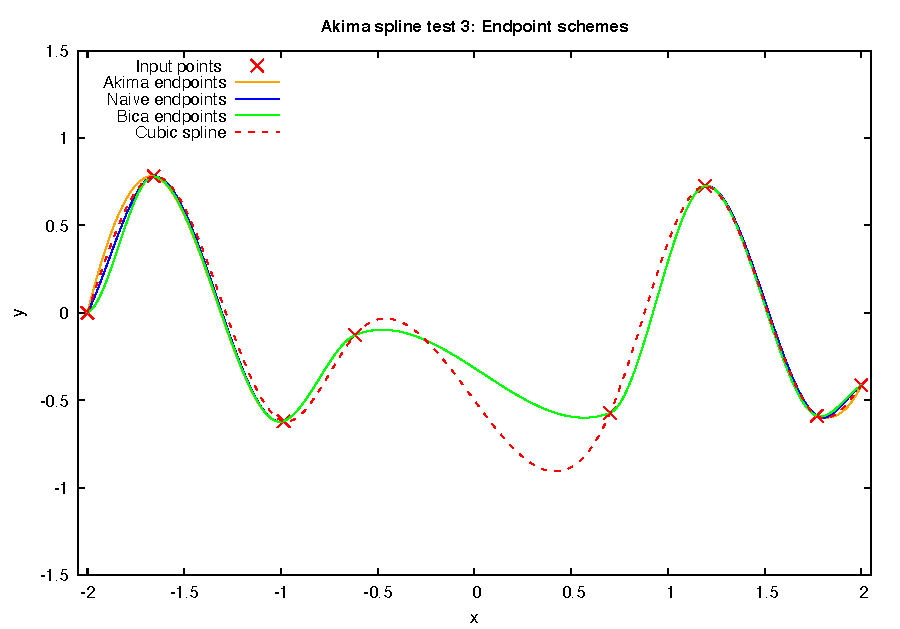
\includegraphics[width=0.9\textwidth]{fig/akima_spline_endpoints.pdf}
    \caption{The three different end-point schemes used on a dataset with irregular oscillations. As expected the difference is only in the first two and last two intervals. The intervals between them are identical. For comparison the cubic spline interpolation is also shown. }
    \label{fig:4}
\end{figure}

\begin{figure}
    \centering
    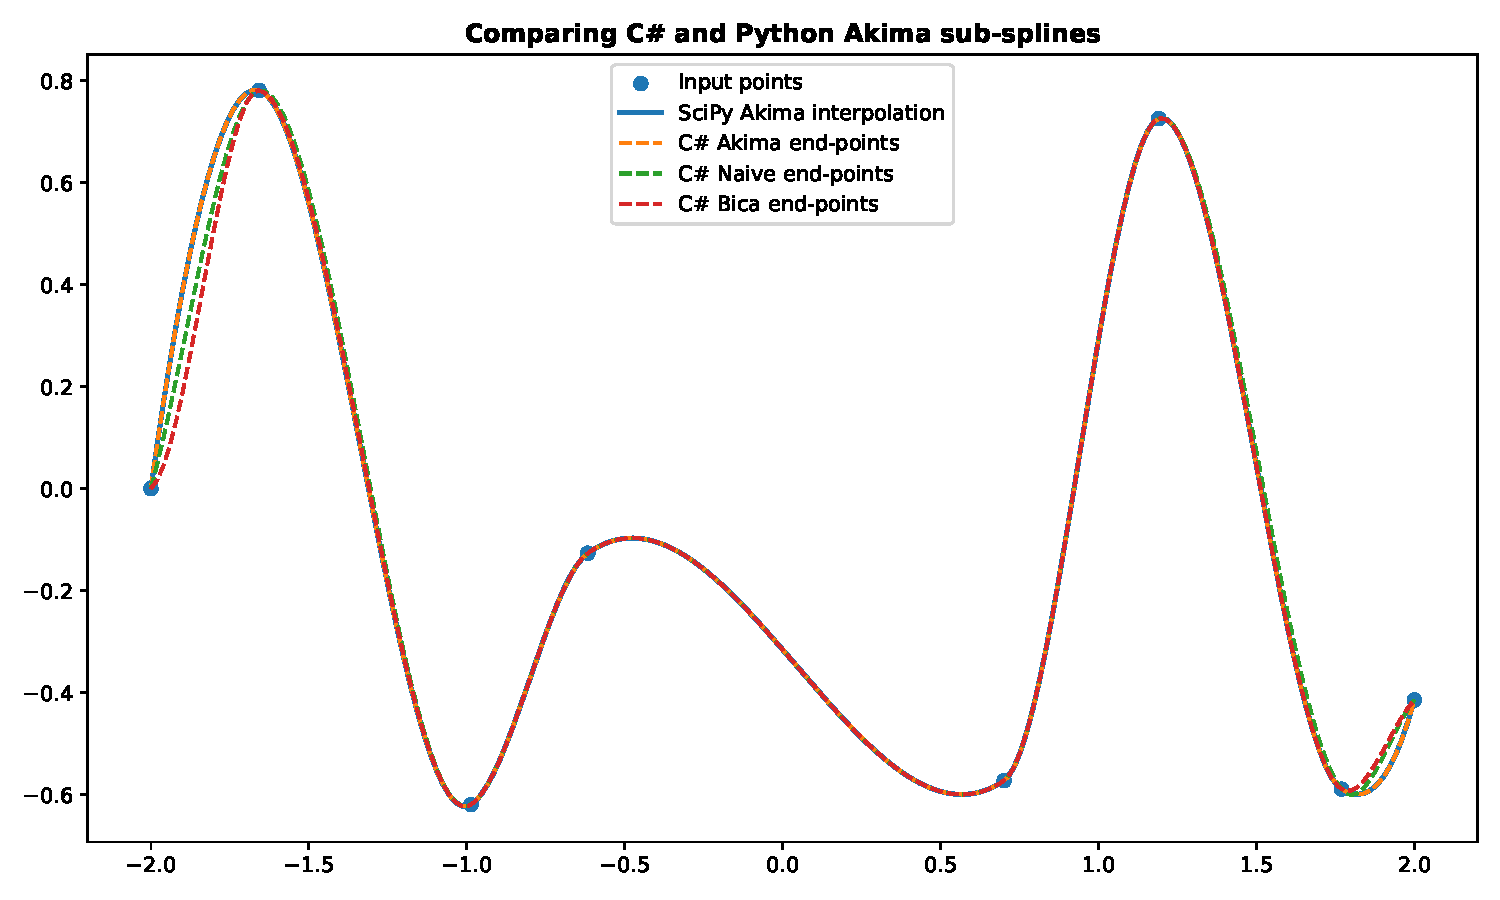
\includegraphics[width=0.9\textwidth]{fig/scipy_comparison.pdf}
    \caption{Comparing the input data set used in \ref{fig:4} with interpolation values from Python's \texttt{scipy.interpolate.Akima1DInterpolator}-routine. First of all the comparison verifies that my routine is calculating the sub-splines correctly. Secondly, I was curious on which end-point scheme is used by \texttt{SciPy}. Not surprisingly it turns out to be Akima's own suggestion of doing the algorithm on a larger set of $p_i$s with two additional elements added at either end.}
    \label{fig:5}
\end{figure}
\end{document}